\subsection{CROSSMINER}

\subsubsection{Open Source Software Challenges}
Open-source software (OSS) is computer software available in source code form, for which the source code and certain other rights are provided under a license that permits users to study, change, and improve the software for free. A report by Standish Group states that adoption of open-source software models has resulted in savings of about 58 billion per year to consumers. Unlike commercial software which is typically developed within the context of a particular organisation with a well-established business plan and commitment to the maintenance, documentation and support of the software, OSS is very often developed in a public, collaborative, and loosely-coordinated manner. This has several implications to the level of quality of different OSS software as well as to the level of support that different OSS communities provide to users of the software they produce.
There are several high-quality and mature OSS projects that deliver stable and well-documented products. Such projects typically also foster a vibrant expert and user community, which provides remarkable levels of support both in answering user questions and in repairing reported defects in the provided software. However, there are also many OSS projects that are dysfunctional in one or more of the following ways:
\begin{itemize}
	\item The development team behind the OSS project invests little time on its development, maintenance and support.
	\item The development of the project has been altogether discontinued due to lack of commitment or motivation.
	\item The documentation of the produced software is limited and/or of poor quality
	\item The source code contains little or low-quality comments which make studying and maintaining it challenging
	\item The community around the project is limited, and questions asked by users receive late/no response and identified defects either get repaired very slowly or are altogether ignored
\end{itemize}
Consequently, developing new software systems by reusing existing open source components raises relevant challenges related to the following activities:
\begin{itemize}
	\item Searching for candidate components.
	\item Evaluating a set of retrieved candidate components to find the most suitable one.
	\item Adapting the selected components to fit the specific requirements.
\end{itemize}


\subsubsection{Selecting Open Source Components}
Deciding whether open source software (OSS) meets the required standards for adoption in terms of quality, maturity, activity of development and user support is not a straightforward process. It involves exploring various sources of information including:
\begin{itemize}
\item Its source code repositories to identify how actively the code is developed, how well the code is commented, whether there are unit tests etc.

\item Communication channels such as newsgroups, forums and mailing lists to identify whether user questions are answered in a timely and satisfactory manner, to estimate the number of experts and users of the software

\item Its bug tracking system to identify whether the software has many open bugs and at which rate bugs are fixed, and

\item Other relevant metadata such as the number of downloads, the license(s) under which it is made available, its release history etc.
\end{itemize}
Dependence on an OSS project can thus either be a blessing or a curse. The ability to accurately assess the risks and benefits of adopting particular OSS projects is essential to the software community at large - especially open source software frameworks and platforms and highly specialised essential utility packages, which can make a depending product or service unexpectedly incur insurmountable technical difficulties when the OSS projects suddenly reach end-of-life.

\subsubsection{Project Technologies}
The overarching aim of CROSSMINER is to deliver an integrated open-source platform that will support the development of complex software systems by (1) enabling monitoring, in-depth analysis and evidence-based selection of open source components, and (2) facilitating knowledge extraction from large open-source software repositories. The six main scientific and technology objectives for the project are the following:
\begin{itemize}
\item Development of source code analysis tools to extract and store actionable knowledge from the source code of a collection of open-source projects

\item Development of natural language analysis tools to extract quality metrics related to the communication channels, and bug tracking systems of OSS projects by using Natural Language Processing and text mining techniques

\item Development of system configuration analysis tools to gather and analyse system configuration artefacts and data to provide an integrated DevOps-level view of a considered open source project

\item Development of workflow-based knowledge extractors that simplify the development of bespoke analysis and knowledge extraction tools shielding engineers from technological issues to concentrate on core analysis tasks

\item Development of cross-project relationship analysis tools to manage a wider range of open source project relationships, such as dependencies and conflicts, based on user-defined similarity measures underpinning the automated creation of project clusters.

\item Development of advanced integrated development environments that will allow developers to adopt the CROSSMINER knowledge base and analysis tools directly from the development environment, while providing alerts, recommendations, and user feedback which will help developers to improve their productivity.
\end{itemize}
The outcomes of the different CROSSMINER analysis tools will contribute to the definition of a knowledge base supporting multidimensional classifications of projects and disclosing a number of applications such as automated identification of complementary and competing projects, project incompatibilities and prediction of the future of given projects based on the evolution of other projects having similar characteristics in the past.

\begin{figure}[H]
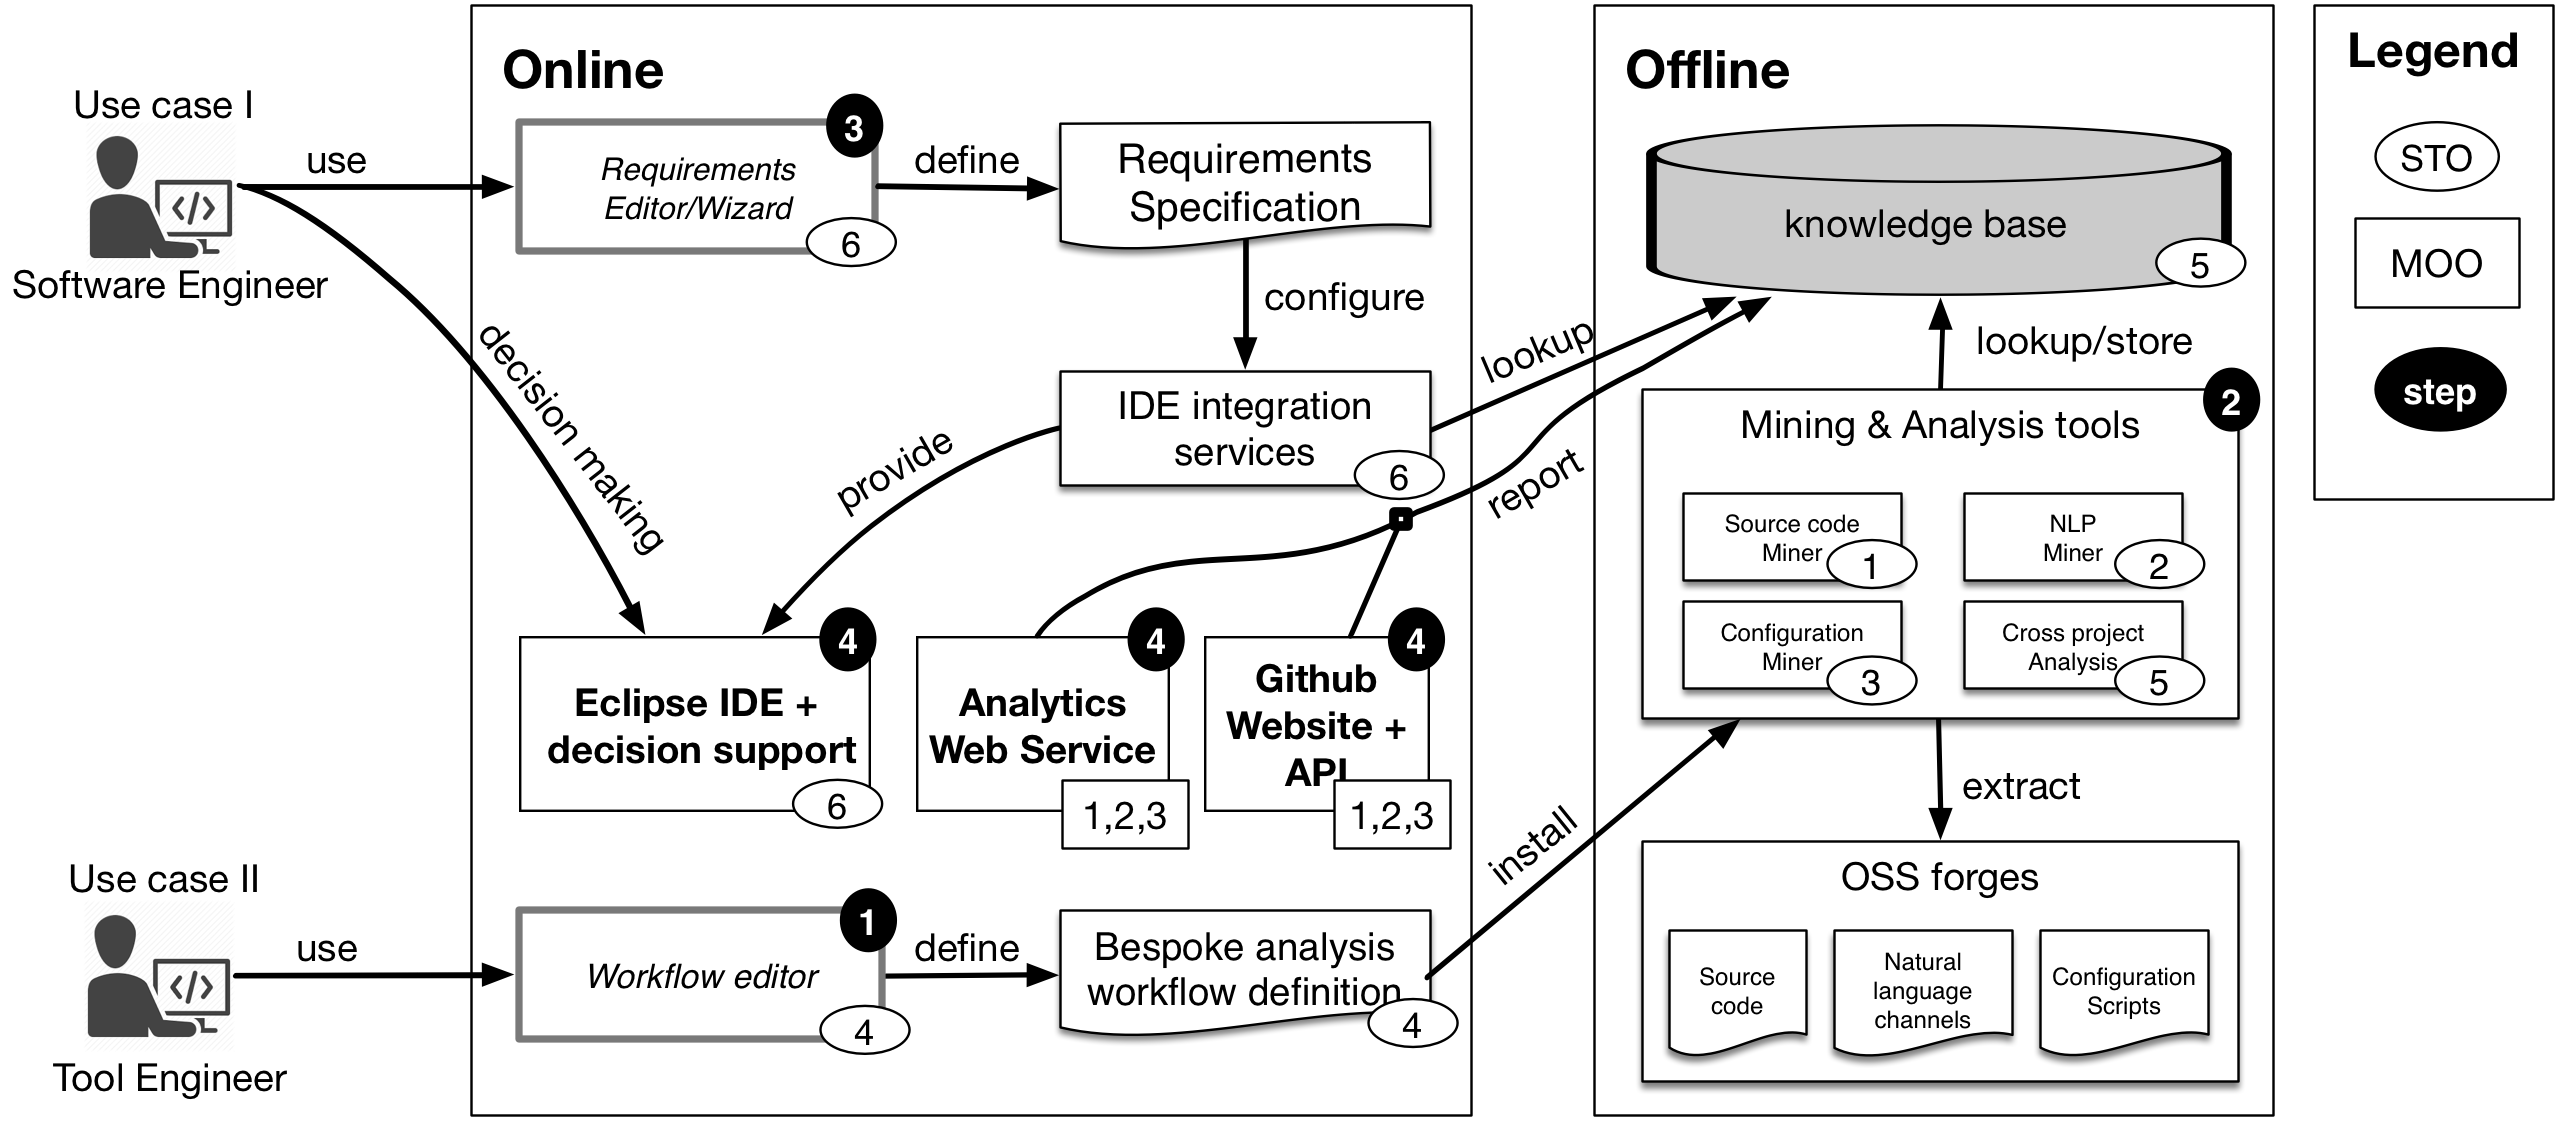
\includegraphics[width=10cm,height=15cm,keepaspectratio]{images/crossminer.png}
\centering
\caption{Crossminer Approach}
\label{fig:CrossminerApproach}
\end{figure}

According to such objectives and the overview about RSSE previously given, CROSSMINER can be seen as a recommendation system aimed at supporting developers while producing new software by integrating existing open source components. Figure \ref{fig:CrossminerApproach} shows CROSSMINER at a glance and how the project aims at reaching its objectives.

Essentially, the \textit{data preprocessing} challenge is addressed by the CROSSMINER components contained in the \texttt{Offline} box shown on the right-hand side of Fig.\ref{fig:CrossminerApproach}. The developer context is captured by the IDE (see the \texttt{Online} box in Fig.\ref{fig:CrossminerApproach}), which also produces recommendations that do not require particular and expensive data analysis. For more elaborated recommendations, preprocessed data available in the \texttt{Knowledge Base} is used. Both the IDE and Web based dashboards will be used to present the produced recommendations to the developer. 

\begin{figure}[H]
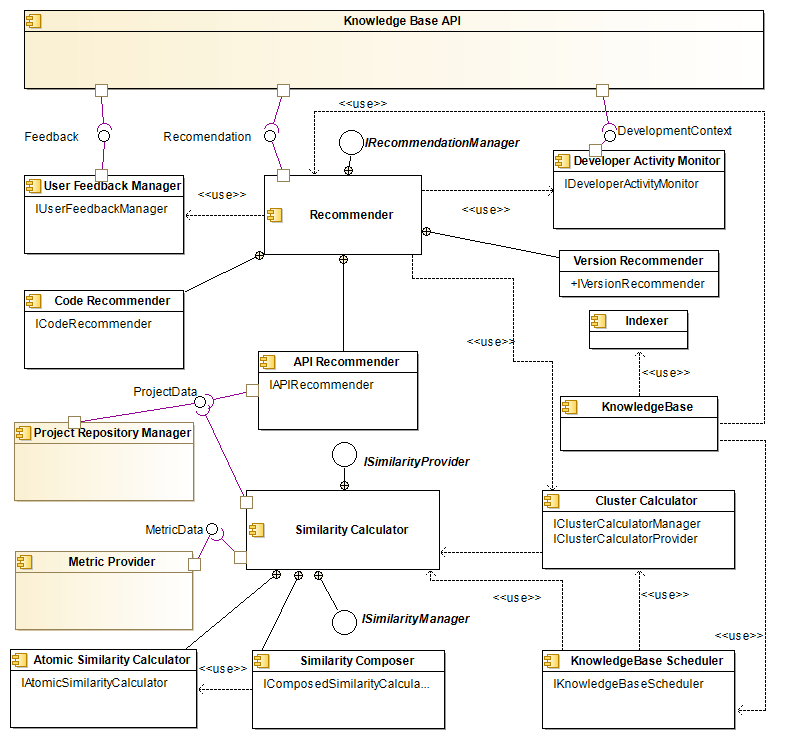
\includegraphics[width=10cm,height=15cm,keepaspectratio]{images/logicView.png}
\centering
\caption{Component Diagram of the Crossminer Knowledge Base}
\label{fig:CrossminerComponent}
\end{figure}

\texttt{KnowledgeBase}  The \textit{KnowledgeBase} component is responsible for setting up the other components, as well as for their execution.

\texttt{Recommender} The \textit{Recommender} component has the responsibility of creating recommendations in response to user requests. This component is extensible in order to add the management of specific kinds of artifacts. The model shows three specific recommender components: the \texttt{CodeRecommender} is able to provide developers with code examples that can be examined to solve the particular problem at hand (e.g., the correct usage of a used API). The \texttt{VersionRecommender} component is able to suggest developers the correct version of a used third party component. The \texttt{APIRecommender} implements the mechanisms for retrieving from the KB information about APIs that should be used in the project being implemented.


\texttt{ClusterCalculator} It has the responsibility of calculating clusters of analyzed artifacts as discussed in the previous sections. To this end similarity functions are used as implemented by the  \texttt{SimilarityCalculator} component, which is in charge of managing the execution of both atomic and composed similarity calculations (see the \texttt{AtomicSimilarityComposer} and
\texttt{SimilarityComposer} components, respectively).

\texttt{KnowledgeBaseScheduler} The calculation of clusters and thus the execution of the available similarity functions is performed periodically and it is triggered by the \textit{KnowledgeBaseScheduler} component.


\texttt{UserFeedbackManager} It manages the feedback expressed by the user on received recommendation. Such a component is used by \texttt{Recommender} to take into account previous user feedback when creating future suggestions. Specific effort will be spent to understand how to identify developers e.g., to remember previous feedback at a user-level.

\texttt{DeveloperActivityMonitor} It stores and manages the data about the activity of the developer while using the CROSSMINER IDE.

\texttt{Indexer} The component implements indexing mechanisms to provide performance gains in the retrieval of data.